\section{Funkcja falowa}

\subsection{Eksperyment z dwoma szczelinami}

Wobrażmy sobie ścianę z dwoma wąskimi otworami oraz drugą równoległą ścianę za nią, która nie ma żadnych otworów.
Teraz wyobraźmy sobie, że osoba strzela kulami we wszystkich kierunkach. Większość kul zatrzymuje się na pierwszej ścianie,
lecz część kul przechodzi przez otwory i trafia na drugą ścianę.
Jakiego obrazu spodziewamy się na drugiej ścianie? Spodziewamy się dwóch kropek, w miejscach odpowiadających otworom na pierwszej ścianie. To też obserwujemy.

\begin{figure}[H]
    \centering
    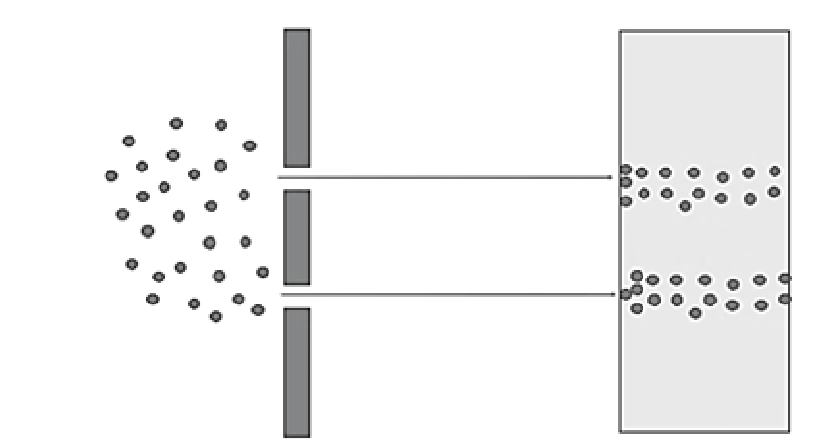
\includegraphics[width=0.5\textwidth]{szczeliny}
    \caption{Eksperyment z dwoma szczelinami. \textit{Źródło: Ranjbar, Vahid. (2023)}}
    \label{fig:szczeliny}
\end{figure}

\subsection{Eksperyment ze światłem}
W roku 1801 Thomas Young przeprowadził podobny eksperyment, ale przepuszczając przez szczeliny światło.
Przez dwie szczeliny przechodziła tak zwana fala płaska, poruszająca się w kierunku ekranu.
W sensie optyki klasycznej albo termodynamiki klasycznej, możemy powiedzieć, że przykładowo światło słoneczne jest taką falą płaską.
Ta fala płaska przechodzi przez szczeliny, a następnie dalej jako fala płaska przemieszcza się w kierunku oddalonego ekranu.

Co zobaczymy na ekranie? Na ekranie zobaczymy coś niespodziewanego - będzie to obraz interferencyjny.
\begin{figure}[H]
    \centering
    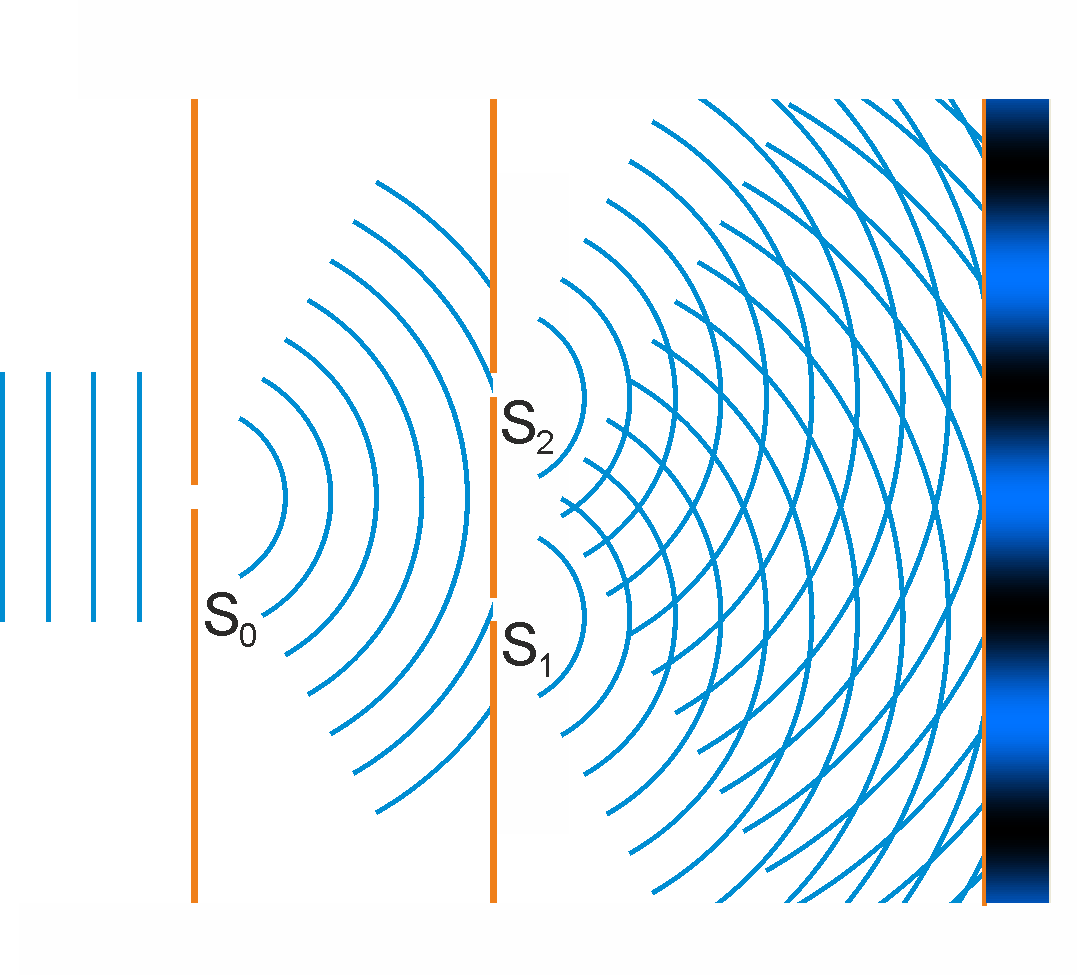
\includegraphics[width=0.5\textwidth]{szczeliny-fale}
    \caption{Eksperyment z dwoma szczelinami. \textit{Źródło: e-Fizyka, AGH}}
    \label{fig:szczeliny-fale}
\end{figure}

Zastanówmy się, w jaki sposób można opisać intensywności światła ukazujące się na ekranie.

Zacznijmy od amplitudy fali (amplitudy światła) - jest to wektor zależny od położenia w przestrzeni oraz czasu:
\begin{equation*}
    A(\bar{r}, t)
\end{equation*}
Intensnywność światła $I$ można zapisać jako kwadrat amplitudy niezależnej od modułu:
\begin{equation*}
    I = |A|^2
\end{equation*}
Następnie pojawia się tak zwana zasada superpozycji. Aby obliczyć amplitudę całkowitą, musimy zsumować amplitudy fal pochodzących z obu szczelin (z obu źródeł):
\begin{equation*}
    \bar{A}(\bar{r}, t) = \bar{A}_1(\bar{r}, t) + \bar{A}_2(\bar{r}, t)
\end{equation*}

Intensywność całkowita będzie przybierać następującą postać:
\begin{equation*}
    I = |A_1|^2 + |A_2|^2 + A_1 A_2^* + A_1^* A_2
\end{equation*}

Człon $A_1 A_2^* + A_1^* A_2$ jest odpowiedzialny za interferencję. Obraz widoczny na ekranie jest spowodowany superpozycją fal pochodzących z obu szczelin.

\subsection{Proste zagadnienie}

Rozważmy najprostsze zagadnienie. W tym zagadnieniu podkreślamy, że odległość między szczelinami $d$ jest mała (dużo mniejsza niż odległość do ekranu $D$).
Na ekranie zaznaczamy pewien punkt $x$ oraz zaznaczamy odległości punktu $x$ od szczelin. Odległość $x$ od szczeliny $1$ wynosi $r_1$, a odległość $x$
od szczeliny $2$ wynosi $r_2$.

\begin{figure}[H]
    \centering
    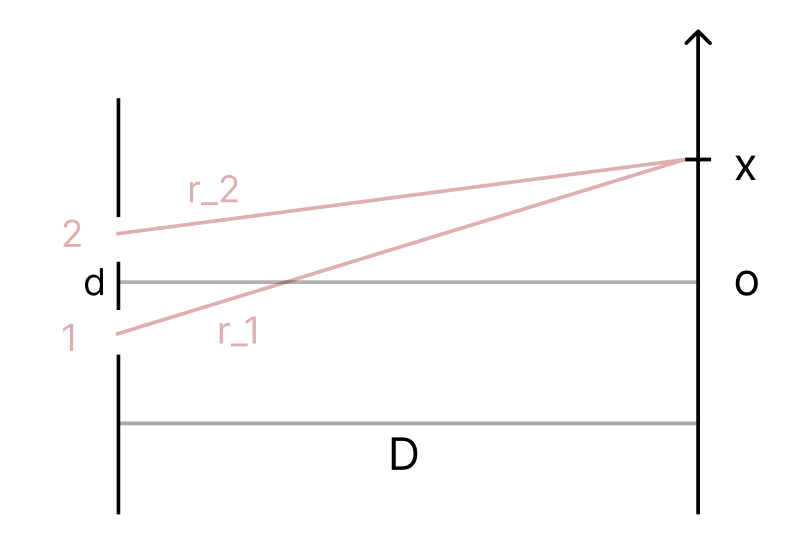
\includegraphics[width=0.5\textwidth]{prosty-eksperyment}
    \caption{Prosty eksperyment.}
    \label{fig:prosty-eksperyment}
\end{figure}

Rozważamy proste fale monochromatyczne, to znaczy amplitudy dla nich mają następującą postać:
\begin{equation*}
    A_1 = a_1 \exp[i(\omega t - \bar{k} \bar{r}_1 + \delta_1)]
\end{equation*}
\begin{equation*}
    A_2 = a_2 \exp[i(\omega t - \bar{k} \bar{r}_2 + \delta_2)]
\end{equation*}

Ponieważ mamy jedno źródło światła, możemy przyjąć, że $a_1 = a_2 = a$ i $\delta_1 = \delta_2 = 0$. 
Symbol $k$ oznacza wektor falowy, który ma kierunek fali. Zapisujemy go jako:
\begin{equation*}
    k = \frac{2\pi}{\lambda}
\end{equation*}
Wersor kierunku fali zapisujemy jako:
\begin{equation*}
    \frac{\bar{k}}{|k|}
\end{equation*}
Przechodzimy do geometrii. Chcemy zrozumieć, jaka będzie intensywność w punkcie $x$ na ekranie.

Wektory $\bar{k}_1$ i $\bar{k}_2$ będą równoległe do siebie, zatem możemy zapisać: $\bar{k}_1 = \bar{k}_2$.


Wyznaczamy $r_1^2$ i $r_2^2$:
\begin{equation*}
    r_1^2 = D^2 + \left(x + \frac{d}{2} \right)^2
\end{equation*}
\begin{equation*}
    r_2^2 = D^2 + \left(x - \frac{d}{2} \right)^2
\end{equation*}
Stąd:
\begin{equation*}
    r_1^2 - r_2^2 = 2xd
\end{equation*}
Ponieważ $r_1$ i $r_2$ są bardzo duże, a różnica między nimi jest mała, możemy zapisać:
\begin{equation*}
    r_1 - r_2 \approx \frac{xd}{D}
\end{equation*}
Intensywność końcowa:
\begin{align*}
    I &= \left(a\cdot e^{i\omega t}\right)^2 \cdot \left[e^{-ikr_1}+e^{-ikr_2}\right]^2 \\
    &= 2 a^2 \left(\cos{\left(kr_1-kr_2\right)}+1\right) \\
    &= 2 a^2 \left(1 + \cos{\left(k(r_1-r_2)\right)}\right) \\
    &= 2 a^2 \left(1 + \cos{\left(\frac{2\pi}{\lambda}\cdot\frac{xd}{D}\right)}\right) = I(x)
\end{align*}

Pytanie - dla jakich $x$ będzie maksymalna intensywność?
Aby znaleźć maksimum, obliczamy pochodną $I(x)$ i przyrównujemy do zera - wartość w zerze będzie albo maksimum, albo minimum.
Chcemy zatem, aby argument cosinusa przyjmował wartość $1$. Będzie to dla $2k\pi$, $k=0,1,2,3,\ldots$. Przyrównując:
\begin{equation*}
    \frac{2\pi}{\lambda} \frac{xd}{D} = 2k\pi
\end{equation*}
Rozwiązując dla $x$ otrzymujemy:
\begin{equation*}
    x_{max} = k \frac{\lambda D}{d}
\end{equation*}
W ten sposób możemy wytłumaczyć obraz interferencyjny - pojawiają się punkty o maksymalnej intensywności
rozłożone wzdłuż osi $x$, a odległość między kolejnymi punktami wynosi $\frac{\lambda D}{d}$.
